\documentclass[11pt]{book}
\frenchspacing
\usepackage{geometry}                % See geometry.pdf to learn the layout options. There are lots.
%\geometry{letterpaper}                   % ... or a4paper or a5paper or ... 
%\geometry{landscape}                % Activate for for rotated page geometry
%\usepackage[parfill]{parskip}    % Activate to begin paragraphs with an empty line rather than an indent
\usepackage{graphicx}
\usepackage{amssymb}
\usepackage{epstopdf}
\DeclareGraphicsRule{.tif}{png}{.png}{`convert #1 `dirname #1`/`basename #1 .tif`.png}

%\usepackage{mystyle}

\usepackage[T1]{fontenc}
\usepackage{ textcomp }


%% LaTeX - Article customise

%%% PACKAGES
\usepackage{booktabs} % for much better looking tables
\usepackage{array} % for better arrays (eg matrices) in maths
%\usepackage{paralist} % very flexible & customisable lists (eg. enumerate/itemize, etc.)
\usepackage{verbatim} % adds environment for commenting out blocks of text & for better verbatim
%\usepackage{subfigure} % make it possible to include more than one captioned figure/table in a single float
\usepackage{amsmath}

\usepackage{hyperref}
\usepackage{makeidx}
\usepackage{color}

% These packages are all incorporated in the memoir class to one degree or another...

%%%% SECTION TITLE APPEARANCE
%\usepackage{sectsty}
%\allsectionsfont{\sffamily\mdseries\upshape} % (See the fntguide.pdf for font help)
%% (This matches ConTeXt defaults)
%
%%%% ToC APPEARANCE
%\usepackage[nottoc,notlof,notlot]{tocbibind} % Put the bibliography in the ToC
%
%\setlength{\headheight}{39pt} %to remove warnings
%
%\usepackage{fancyhdr} %to insert logo on the left head of each page
%\pagestyle{fancy}
%%\begin{titlepage}
%\rhead{\includegraphics[width=35mm]{KaSim-logo.png}}
%%\end{titlepage}

\def\KaSim{\textsf{KaSim}}
\def\sep{\hbox{-}}
\def\int{\hbox{\texttt{\~}}}
\def\tcb#1{\textcolor{blue}{\ttt{#1}}}
\def\ttt#1{\texttt{#1}}

\makeindex

%% END Article customise

%%%% added by Vincent to compensate for the lack of mystyle.sty
\frenchspacing
\def\rar{\rightarrow}
\def\ka{\kappa}
\def\ga{\gamma}
\def\bs{\backslash}
\def\noi{\noindent}
\def\ie{ie }
\def\via{via }
\def\set#1{\{#1\}}
\def\ITE#1{\begin{itemize}#1\end{itemize}}
\def\ENU#1{\begin{enumerate}#1\end{enumerate}}
\def\mit#1{{\mathit #1}}
\def\Real{\mathbb R}
\def\Nat{\mathbb N}
\def\dd{-\hspace{0.001cm}-}

%%%%
\def\version{v3}


\title{KaSim reference manual \version}
\author{\url{KappaLanguage.org}}

%\date{}                                           % Activate to display a given date or no date
\begin{document}
\maketitle

\begin{center}
\includegraphics[width=80mm]{img/wip.jpg}
\vspace{3cm}
\\This document is work in progress...
\end{center}

\tableofcontents

\chapter{Introduction}
\begin{center}\includegraphics[width=11cm]{img/KaSim-logo.png}\end{center}

\section{Preamble}
This manual describes the usage of \KaSim, the latest implementation of Kappa, one member of the growing family of rule-based languages. Rule-based modelling has attracted recent attention in developing biological models that are concise, comprehensible, and easily extensible. 
Although this manual contains a self-contained description of Kappa, it is \emph{not} intended as a tutorial on rule-based modeling.%%Therefore, in the following of this manual some familiarity with Kappa is assumed and 
%
\footnote{For an idea of how Kappa is used in a modeling context, the reader might find the following short note useful \href{http://www.pps.jussieu.fr/~danos/pdf/eov.pdf}{Agile modelling of cellular signalling (SOS'08)}. A longer article, expounding on the causal aspects of modeling, is also available: \href{http://www.pps.jussieu.fr/~danos/pdf/ka-fix.pdf}{Rule-based modelling of cellular signalling (CONCUR'07)}, See also this tutorial: \href{http://www.pps.jussieu.fr/~danos/pdf/mytdg.pdf}{Modelling epigenetic information maintenance: a Kappa tutorial (CAV'09)}. 
}%Further explanations, resources and tools can be found there: \url{http://KappaLanguage.org}. 



\section{The \KaSim~engine}
\KaSim~is an open source stochastic simulator of rule-based models~\cite{DanLan04,Dan_etal07a,Fae_etal05} written in the $\ka$-calculus. Basically \KaSim~takes one or several \hyperref[chap:kappa]{kappa files} as input and generates stochastic trajectories of various observables. \KaSim~implements Danos and Krivine's simulation algorithm~\cite{Dan_etal07b} which adapts Gillespie's algorithm~\cite{Gil76,Gil77} to rule-based models. 

A \emph{simulation event}\index{event} corresponds to the application of a rewriting rule, contained in the kappa files, to the current graph\index{graph} (also called a \emph{mixture}\index{mixture}). The rule is selected according to its \emph{activity}\index{activity}, \ie the number of instances it has in the current mixture\index{mixture}, multiplied by its kinetic rate\index{kinetic rate}, and applied to one of its possible instances in the graph. It results in a new graph together with an updated activity\index{activity} for all rules (see Fig.~\ref{fig:event-loop}). Importantly, the cost of a simulation event is independent of the size of the graph it is applied to~\cite{Dan_etal07b}. 

\begin{figure}[htbp]
\begin{center}
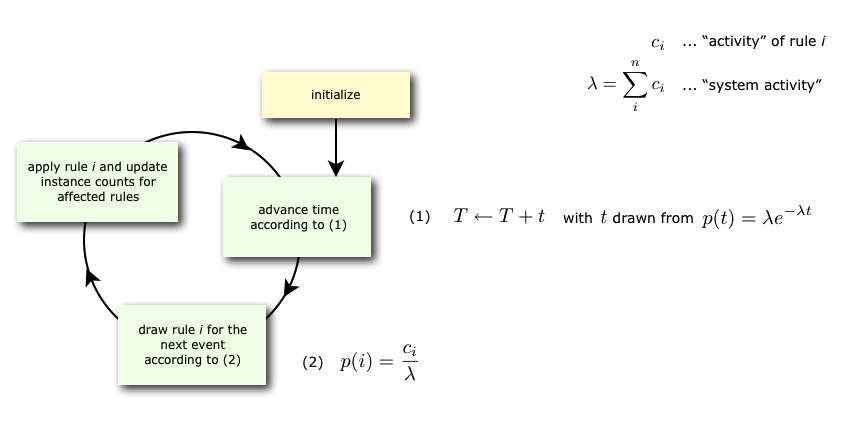
\includegraphics[width=14cm]{img/event-loop.png}
\caption{The event loop}
\label{fig:event-loop}
\end{center}
\end{figure}

Note that \KaSim~is not equipped with a curve visualization tool. However, data outputs are given in a text format that is readily usable by any standard plotting software such as \href{http://www.gnuplot.info/}{gnuplot}.

\section{Support}
\ITE{
\item[-] Kappa language tutorials and downloads: \url{http://kappalanguage.org}
\item[-] Bug reports should be posted on github: \url{https://github.com/jkrivine/KaSim/issues}
\item[-] Questions and answers on the kappa-user mailing list: \url{http://groups.google.com/group/kappa-users}
\item[-] Want to contribute to the project? \ttt{jkrivine} at \ttt{pps} dot \ttt{jussieu} dot \ttt{fr}
}

\chapter{Installation}\label{chap:install}

\section{Using precompiled binaries}
The easiest way to use \KaSim~is to use pre-compiled versions available at \url{https://github.com/jkrivine/KaSim/downloads}. Download the version that corresponds to your operating system (Windows, Linux or Mac OSX) and rename the downloaded file into \KaSim. Note that on Mac OSX or linux it might be necessary to give executable permissions to \KaSim. This can be done using the shell command:  
\ttt{chmod u+x KaSim}. 

To test whether your program does work, simply type \ttt{./KaSim \dd version} on a terminal, from the directory that contains the binaries. If the version is displayed it means that the binaries are indeed compatible with your OS. Otherwise, check that you gave the executable permissions to \KaSim~(see above). Otherwise you may need to compile \KaSim~from the sources (see next Section).

\section{Obtaining the sources}
To obtain \KaSim~you can either use pre-compiled binaries (see previous section) or compile the sources for your architecture. To do so, download the source code from \url{https://github.com/jkrivine/KaSim} and make sure you have a recent ocaml compiler installed. From a terminal window type \ttt{ocamlopt.opt -v}. If nothing appears then you need to install Ocaml Native compiler that can be downloaded from \url{http://caml.inria.fr/download.en.html}. 

\section{Compilation}
Once Ocaml is safely installed, untar \KaSim~archive and compile following these few steps:
\ITE{
\item[\$]\ttt{tar xzvf kasim.tar.gz -d Kappa}
\item[\$]\ttt{cd Kappa}
\item[\$]\ttt{make}
}
At the end of these steps you should see, in the \ttt{Kappa} directory, an executable file named KaSim.  In order to check the compilation went fine, simply type $.\bs$\ttt{KaSim -\,-version}. If the ocaml native compiler \ttt{ocamlopt.opt} is not in the path of your system, you may set the variable \ttt{OCAMLBINPATH} to point to the location of the compiler by editing the corresponding line in the Makefile.

\chapter{The command line}\label{chap:cl}

\section{General usage}
From a terminal window, \KaSim~can be invoked by typing 
\ITE{
\item[\$] \ttt{KaSim -i file\_1 ... -i file\_n [option] }
}
where \ttt{file\_i} are the input kappa files containing the rules, initial conditions and observables, see Chapter~\ref{chap:kappa} below. Tables~\ref{tab:options} and \ref{tab:add-options} summarize all the options that can be given to the simulator. Basically, one specifies an upper bound either in bio time (arbitrary time unit), or in number of events. Note that bio-time is computed using Gillespie's formula for time advance (see Fig.~\ref{fig:event-loop}) and should not be confused with CPU-time (it's not even proportional). In doubt, we recommend using a bound in number of events since the cost of one event application is bounded (in CPU time) by a constant, so the simulation time of $n$ events is roughly $k$ times faster than a simulation of $k*n$ events.

\section{Main options}

Table~\ref{tab:options} summarizes the main options that are accessible through the command line. Options that expects an argument are preceded by a single dash, options that do not need any argument start with a double dash. Note that the option \ttt{-p} specifies the number of points that one wishes to have in the final plot. The interval at which these points will be taken is then computed using the simulation limit defined by the user using option \ttt{-t} or \ttt{-e}. For instance requiring a simulation of 100 points during 10 time units will result in a simulation where observables are recorded every 0.1 time units, while requiring 100 points for 1000 events will result in observable being written every 10 events (be careful that the event density, \ie the number of events per time unit, might vary during a simulation, and thus the two sampling methods can lead to very different repartitions of the moments at which observables are recorded even if they sepecify the same number of observations). 

The results of the options \ttt{-im} and \ttt{-flux} is explained in Chapter~\ref{chap:advanced}. 

\begin{table}[htdp]
\caption{Command line: main options}
\begin{center}
\begin{tabular}{|l|l|}
\hline 
Argument & Description \\ \hline
\ttt{-e $e_\mit{max}$} & Terminates simulation after $e_\mit{max}\geq 0$ events\\
\ttt{-t $t_\mit{max}$} & Terminates simulation after $t_\mit{max}\geq 0.0$ time units\\
\ttt{-p $n$} & Produces a data file\index{data file} (default: \ttt{data.out}) with $n\geq 0$ data points\\
\ttt{-o} \textit{file} & Set the name of data file to \textit{file}\\ 
\ttt{-d} \textit{dir} & Output any produced file to the directory \textit{dir}\\
\hline
\end{tabular}
\end{center}
\label{tab:options}
\end{table}%

\section{Advanced options}

Table~\ref{tab:add-options} summarizes the advanced options that are accessible through the command line.

\begin{table}[htdp]
\caption{Command line: advanced options}
\begin{center}
\begin{tabular}{|l|l|}
\hline 
Argument & Description \\ \hline
\ttt{\small -seed $n$} &\small Seeds the pseudo-random number generator $n>0$ \\
\ttt{\small \dd implicit-signature} &\small Automatically deduce agent signatures (see Chapter~\ref{chap:advanced})\\
\ttt{\small -im} \textit{file} &\small Produces a dot format file of the decorated influence map \\
\ttt{\small -flux} \textit{file} &\small Produces a dot format file of the activation/inhibition flux \\ & measured during the simulation \\
\ttt{\small -make-sim} \textit{sim\_file} &\small makes a simulation package out of the input kappa files \\
\ttt{\small -load-sim} \textit{sim\_file} &\small use simulation package \textit{sim\_file} as input\\
\ttt{\small \dd gluttony} &\small simulation mode that is memory intensive \\ &\small but that speeds up simulation time\\

\hline
\end{tabular}
\end{center}
\label{tab:add-options}
\end{table}%
%
\section*{Example}
The command 
\ITE{
\item[\$] \ttt{KaSim -i model.ka -e 1000000 -p 1000 -o model.out}  
}
will generate a file \ttt{model.out} containing the trajectories of the observables defined in the kappa file \ttt{model.ka}. The file \ttt{model.out} will contain 1000 data points (\ie in this case, a measure will be taken every 1000 events). The command
\ITE{
\item[\$] \ttt{KaSim -i init.ka -i rules.ka -i obs.ka -i mod.ka -t 1.5 -p 1000}  
}
will generate a file \ttt{data.out} (default name) containing 1000 data points of a simulation of 1.5 seconds (arbitrary time units) of the model. Note that the input kappa file is split in 4 files containing, for instance, the initial conditions, \ttt{init.ka}, the rule set, \ttt{rules.ka}, the observables, \ttt{obs.ka}, and the perturbations, \ttt{pert.ka} (see Chapter~\ref{chap:kappa} for details). The order in which the files are given does not matter.

\section*{The activation and flux maps}

The command line options \ttt{-im} and \ttt{-flux} allows modelers to generate additional information about the statics and the dynamics of the model that is being considered (see Chapter~\ref{chap:advanced}).

\chapter{The kappa file}\label{chap:kappa}

\section{General remarks}
The \emph{Kappa File}\index{kappa file} (KF) is the formal representation of your model. We use KF to denote the union of the files that are given as input to \KaSim~(argument \ttt{-i}). Each line of the KF is interpreted by \KaSim~as a \emph{declaration}\index{declaration}. If the line is ended by the escape character '\ttt{$\bs$}' the continuation of the declaration is parsed onto the next line. Declarations can be of 5 types: \emph{signatures} (Sec.~\ref{sec:sig}), \emph{rules}\index{rule} (Sec.~\ref{sec:rules}), \emph{variables}\index{variable} (Sec.~\ref{sec:var}), \emph{initial conditions}\index{initial condition} (Sec.~\ref{sec:init}), \emph{perturbations}\index{perturbation} (Sec.~\ref{sec:mod}) and \emph{parameter configurations} (Sec.~\ref{sec:param}). The KF's structure is quite flexible and can be divided in any number of sub-files in which the order of declarations does not matter (to the exception of variable declarations, see Section~\ref{sec:var} for details). Comments\index{comments} can be used by inserting the marker \ttt{\#} that tells \KaSim~to ignore the rest of the line. 

\section{Agent signature}\label{sec:sig}
%
\emph{Agent signatures}\index{agent signature} constitute a form of typing information about the agents that are used in the model. It contains information about the name and number of interaction sites the agent has, and about their possible internal states. A signature is declared in the KF by the following line:
\ITE{
\item[] \ttt{\%agent: } \textit{signature\_expression}
}
according to the grammar given in Table~\ref{tab:sig}.
%%
\begin{table}[htbp]
  \centering
  \begin{tabular}{@{} lcl @{}}
    \textit{signature\_expression} & ::= & \tcb{Id}\tcb{(}\textit{sig}\tcb{)} \\ 
    \textit{sig} & ::= & \tcb{Id}~\textit{internal\_state\_list}\tcb{,}\ \textit{sig} $\mid\varepsilon$ \\ 
    \textit{internal\_state\_list} & ::= & \tcb{\int Id}~\textit{internal\_state\_list} $\mid\varepsilon$
    \end{tabular}
  \caption{Agent signature expression: terminal symbol are denoted in (blue) typed font. Symbol \ttt{Id} can be any string generated by regular expression $[a\sep z\ A\sep Z\ 0\sep 9][a\sep z\ A \sep Z\ 0\sep 9\ \_ \ -]^*$. Terminal symbol $\varepsilon$ stands for the empty symbol.}
  \label{tab:sig}
\end{table}
%%
For instance the line:
\ITE{
\item[] \ttt{\%agent: A(x,y\int u\int p,z\int 0\int 1\int 2) \# Signature of agent A} 
}
will declare an agent \ttt{A} with 3 \emph{(interaction) sites} \ttt{x,y} and \ttt{z} with the site \ttt{y} possessing two \emph{internal states}\index{internal state} \ttt{u} and \ttt{p} (for instance for the unphosphorylated and phosphorylated forms of \ttt{y}) and the site \ttt{z} having possibly 3 states respectively 0, 1 and 2. Note that internal states\index{internal state} values are treated as untyped symbols by \KaSim, so choosing a character or an integer as internal state is purely matter of convention. 

\section{Rules}\label{sec:rules}

Once agents are declared, one may add to the KF the rules\index{rule} that describe their dynamics through time. Roughly a Kappa rule looks like 
\ITE{
\item[] \ttt{`my rule'} {\it kappa\_expression} $\rar$ {\it kappa\_expression} \ttt{@} {\it rate\_expression}  
}
where \ttt{`my rule'} can be any name that will refer to the subsequent rule that can be decomposed into a \emph{left hand side}\index{left hand side} (LHS) and a \emph{right hand side}\index{right hand side} (RHS) kappa expressions\index{kappa expressions} together with a \emph{kinetic rate expression} \index{kinetic rate}. Kappa and rate expressions are generated by the grammar given in Table~\ref{tab:patterns}.
%%
\begin{table}[htbp]
  \centering
  \begin{tabular}{@{} lcl @{}}
    \textit{kappa\_expression} & ::= & \textit{agent\_expression} \tcb{,} \textit{kappa\_expression} $\mid\varepsilon$ \\ 
    \textit{agent\_expression} & ::= &  \tcb{Id}\tcb{(}\textit{interface}\tcb{)} \\
    \textit{interface} &::=& $\varepsilon\mid$ \tcb{Id} \textit{internal\_state link\_state}\\
    \textit{internal\_state} &::=& $\varepsilon$ | \tcb{\int Id} \\
    \textit{link\_state} &::=& $\varepsilon$ | \tcb{!n} | \tcb{!\_} | \tcb{?}  \\\\
    \textit{rate\_expression} &::=& $\ga$ | $\ga$\tcb{(}$k$\tcb{)} 
    \end{tabular}
  \caption{Kappa expressions: In addition to the conventions of Table~\ref{tab:sig}, symbol \ttt{n} denotes any positive integer and $\ga,k$ are any positive real number.}
  \label{tab:patterns}
\end{table}
%%
\subsection{A simple rule}
With the signature of \ttt{A} defined in the previous section, the line
\ITE{
\item[] \ttt{`A dimerization' A(x),A(y\int p)} $\rar$ \ttt{A(x!1),A(y\int p!1) @ $\ga$} 
}
denotes a dimerization rule between two instances of agent \ttt{A} provided the second is phosphorylated (say that is here the meaning of \ttt{p}) on site \ttt{y}. Note that the bond between both \ttt{A}s is denoted by the identifier \ttt{!1} which uses an arbitrary integer (\ttt{!0} would denote the same bond. In Kappa, a bond may connect exactly 2 sites so any occurrence of a bond identifier \ttt{!}$n$ has to be paired with exactly one other sibling in the expression. Note also the fact that site \ttt{z} of \ttt{A} is not mentioned in the expression which means that it has no influence on the triggering of this rule. This is the \emph{don't care don't write convention} (DCDW) \index{don't care don't write} that plays a key role in resisting combinatorial explosion when writing models.

\subsection{Adding and deleting agents}
Sticking with \ttt{A}'s signature, the rule
\ITE{
\item[] \ttt{`budding A' A(z)} $\rar$ \ttt{A(z!1),A(x!1) @ $\ga$ } 
}
indicates that an agent \ttt{A} free on site \ttt{z}, no matter what its internal state is, may beget a new copy of \ttt{A} bound to it \via site \ttt{x}. Note that in the RHS, agent \ttt{A}'s interface is not completely described. Following the DCDW convention\index{don't care don't write}, \KaSim~will then assume that the sites that are not mentioned are created in the \emph{default state}\index{default state}, \ie they appear free of any bond and their internal state (if any) is the first of the list shown in the signature (here state \ttt{u} for \ttt{y} and \ttt{0} for \ttt{z}).

Importantly, \KaSim~respects the \emph{longest prefix convention}\index{longest prefix convention} to determine which agent in the RHS stems from an agent in the LHS. 
In a word, from a rule of the form $a_1,\dots,a_n\rar b_1,\dots,b_k$, with $a_i$s and $b_j$s being agents, one computes the biggest indices $i\leq n$ such that the agents $a_1,\dots,a_i$ are pairwise consistent with $b_1,\dots,b_i$, \ie the $a_j$s and $b_j$s have the same name and the same number of sites. In which case we say that the for all $j\leq i$, $a_j$ is \emph{preserved} by the transition and for all $j>i$, $a_j$ is \emph{deleted} by the transition and $b_j$ is \emph{created} by the transition. This convention allows us to write a deletion rule as:
\ITE{
\item[] \ttt{`deleting A' A(x!1),A(z!1)} $\rar$ \ttt{A(x) @ $\ga$} 
}
which will remove the \ttt{A} agent in the mixture that will match the second occurrence of \ttt{A} in this rule.

\subsection{Side effects}\label{sec:side-effect}

It may happen that the application of a rule has some \emph{side effects}\index{side effect} on agents that are not mentioned explicitly in the rule. Consider for instance the previous rule:
\ITE{
\item[] \ttt{`deleting A' A(x!1),A(z!1)} $\rar$ \ttt{A(x) @ $\ga$} 
}
The \ttt{A} in the graph that is matched to the second occurrence of \ttt{A} in the LHS will be deleted by the rule. As a consequence all its sites will disappear together with the bonds that were pointing to them. For instance, when applied to the graph 
\ITE{
\item[] $G=$\ttt{A(x!1,y\int p,z\int2),A(x!2,y\int u,z\int0!1),C(t!2)}
} 
the above rule will result in a new graph $G'=\ttt{A(x!1,y\int p,z\int2),C(t)}$ where the site \ttt{t} of \ttt{C} is now free as side effect.

\emph{Wildcard} symbols for link state \ttt{?} (for bound or not), \ttt{!\_} (for bound to someone), may also induce side effects when they are not preserved in the RHS of a rule, as in
\ITE{
\item[] \ttt{`Disconnect A' A(x!\_)} $\rar$ \ttt{A(x) @ $\ga$} 
}
or 
\ITE{
\item[] \ttt{`Force bind A' A(x?)} $\rar$ \ttt{A(x!1),C(t!1) @ $\ga$} 
}
%%
Both these rule will cause \KaSim~to raise a warning at rule compilation time.

\subsection{Rates}\label{sec:kinetics}
As said earlier, $\ka$ rules are equipped with one or two \emph{kinetic rate(s)}\index{kinetic rate}. A rate is a real number called the \emph{individual-based or stochastic rate constant}\index{kinetic rate!stochastic rate constant}, it is the rate at which the corresponding rule is applied per instance of the rule. Its dimension is the inverse of a time $[T^{-1}]$.

The stochastic rate is related to the \emph{concentration-based rate constant}\index{kinetic rate!deterministic rate constant} $k$ of the rule of interest by the following relation:
%corrected by the volume $V$ in which the model is considered. 
%
%%We often want to express $\ga$ in ``per molecule'' rather than ``per mole''. 
%%This only changes the numerical value, not the dimension (both are numbers of molecules): 
%
%%The relation between both rate constant is:
\begin{equation}\label{stochrate}
k = \ga{({\cal A}\; V)^{(a-1)}} %\qquad [\mathit{molecule}^{-1} \mathit{s}^{-1}],
\end{equation}
where 
$V$ is the volume where the model is considered,
${\cal A}= 6.022\cdot 10^{23}$ is Avogadro's number, %number of $H$ atoms needed to make up for a gram of $H$, 
$a\geq0$ is the arity of the rule (\ie 2 for a bimolecular rule).

In a modeling context, the constant $k$ is typically expressed using \emph{molars} $M:=\mit{moles}\,l^{-1}$ (or variants thereof such
as $\mu M$, $nM$), and seconds or minutes. If we choose molars and seconds, $k$'s unit is $\mathit{M}^{1-a}\mathit{s}^{-1}$, as 
follows from the relation above.

Concentration-based rates are usually favored for measurements and/or deterministic models, so it is useful to know how to convert them into
individual-based ones used by KaSim. 
%We refer the reader to \url{http://www.KappaLanguage.org} for a tutorial on kinetic rates. 
Here are typical volumes used in modeling:
\begin{itemize}
\item
Mammalian cell: $V=2.25\; 10^{-12}l$  ($1l=10^{-3}m^3$), and ${\cal A}V=1.35\; 10^{12}$. 

A concentration of $1M$ in a mammalian cell volume corresponds to $1.35\; 10^{12}$ molecules; $1nM\approx 1350$ molecules per cell.
\item
Yeast cell (haploid): $V=4\; 10^{-14}l$, and ${\cal A}V=2.4\; 10^{10}$. 

A concentration of $1M$ in a yeast cell volume corresponds to $2.4\; 10^{10}$ molecules; $1nM\approx 24$ molecules per cell. The volume is doubled in a diploid cell.
\item
E.\@ Coli cell: $V=10^{-15}l$, and ${\cal A}V=10^{8}$. 

A concentration of $1M$ in a yeast cell volume corresponds to $10^{8}$ molecules; $10nM\approx 1$ molecule per cell.
\end{itemize}

The table below lists typical ranges for deterministic rate constants and 
their stochastic counterparts assuming a mammalian cell volume.

\begin{table}[htbp]
\centering
\begin{tabular}{@{} lllr @{} }
\toprule
process & $k$ & $\gamma$ %& stoch. dimension
\\
\midrule
general binding & $10^{7}-10^{9}$ & $10^{-5}-10^{-3}$ %& $s^{-1}$ %$molecule^{-1} s^{-1}$
\\
general unbinding &  $10^{-3} - 10^{-1}$ & $10^{-3}-10^{-1}$ %& $s^{-1}$
\\
dephosphorylation & 1 & 1 %& $s^{-1}$
\\
phosphorylation & 0.1 & 0.1 %& $s^{-1}$
\\
receptor dimerization & $2\; 10^{6}$ & $1.6 \;10^{-6}$ %& $s^{-1}$%$molecule^{-1} s^{-1}$
\\
receptor dissociation & $1.6\; 10^{-1}$ & $1.6\; 10^{-1}$ %& $s^{-1}$
\\
\bottomrule
\end{tabular}
\end{table}

\subsection{Ambiguous molecularity}\label{sec:ambiguous}

It is considered malpractice to use a $\ka$-rule of the form \ttt{A(x),B(y)$\rar \dots$ @ $\ga$} in a model where this rule could be applied in a context where \ttt{A} and \ttt{B} are sometimes already connected and sometimes disconnected. Indeed, this would lead to an inconsistency in the definition of the kinetic rate $\ga$ which should have a volume dependency in the former case and no volume dependency in the latter (see Section~\ref{sec:kinetics}). 

This sort of ambiguity should be resolved, if possible, by refining the ambiguous rule into cases that are either exclusively unary or binary. Each refinement having a kinetic rate that is consistent with its molecularity. Note that in practice, for models with a large number of agents, it is sufficient to assume that the rule \ttt{A(x),B(y)$\rar \dots$ @ $\ga$} will have only binary instances. In this case it suffices to consider the approximate model:
\begin{itemize}
\item[]\ttt{`assumed binary AB' A(x),B(y)$\rar \dots$ @ $\ga_2$}
\item[]\ttt{`unary AB' A(x,c!1),C(a!1,b!2),B(y,c!2)$\rar \dots$ @ $k_1$}
\end{itemize}

There are however systems where even enumerating unary cases becomes impossible. As an alternative, one should use the kappa notation for ambiguous rules: 
\ITE{
\item[] \ttt{`my rule'} {\it kappa\_expression} $\rar$ {\it kappa\_expression} \ttt{@} $\ga_2(k_1)$  
}
which will tell \KaSim~to apply the above rule with a rate $\ga_2$ for binary instances and a rate $k_1$ for unary instances. The obtained model will behave exactly as a model in which the ambiguous rule has been replaced by unambiguous refinements. However the usage of such rule might \emph{slowdown simulation in a significant manner} depending on various parameters (such as the presence of large polymers in the model). We give below an example of a model utilizing binary/unary rates for rules\footnote{This model is available in the source repository \ttt{model/poly.ka}.}.

{\tt\footnotesize
\begin{enumerate}
\item \%agent: A(b,c)
\item \%agent: B(a,c)
\item \%agent: C(b,a)
\item \#\#
\item \%var: `V' 1
\item \%var: `k1' [inf]
\item \%var: `k2' 1.0E-4/`V'
\item \%var: `k\_off' 0.1
\item \#\#
\item `a.b' A(b),B(a) -> A(b!1),B(a!1) @ `k2'(`k1')
\item `a.c' A(c),C(a) -> A(c!1),C(a!1) @ `k2'(`k1')
\item `b.c' B(c),C(b) -> B(c!1),C(b!1) @ `k2'(`k1')
\item \#\#
\item `a..b' A(b!a.B) -> A(b) @ `k\_off'
\item `a..c' A(c!a.C) -> A(c) @ `k\_off'
\item `b..c' B(c!b.C) -> B(c) @ `k\_off'
\item \#\#
\item \%var: `n' 1000
\item \#\#
\item \%init: `n' A,B,C
\item \%mod: [E] > 10000 do \$STOP 
\end{enumerate}
}

Notice at lines 10-12 the use of binary/unary notation for rules. As a result binding between between freely floating agents will occur at rate \ttt{`k2'} while binding between agents that are part of the same complex will occur at rate \ttt{`k1'}. Line 21 contains a \emph{perturbation} that requires \KaSim~to stop the simulation after 10,000 events and output the list of molecular species present in the final mixture (see Section~\ref{sec:mod}) and that we give Figure~\ref{fig:species}.

\begin{figure}[htbp]
\begin{center}
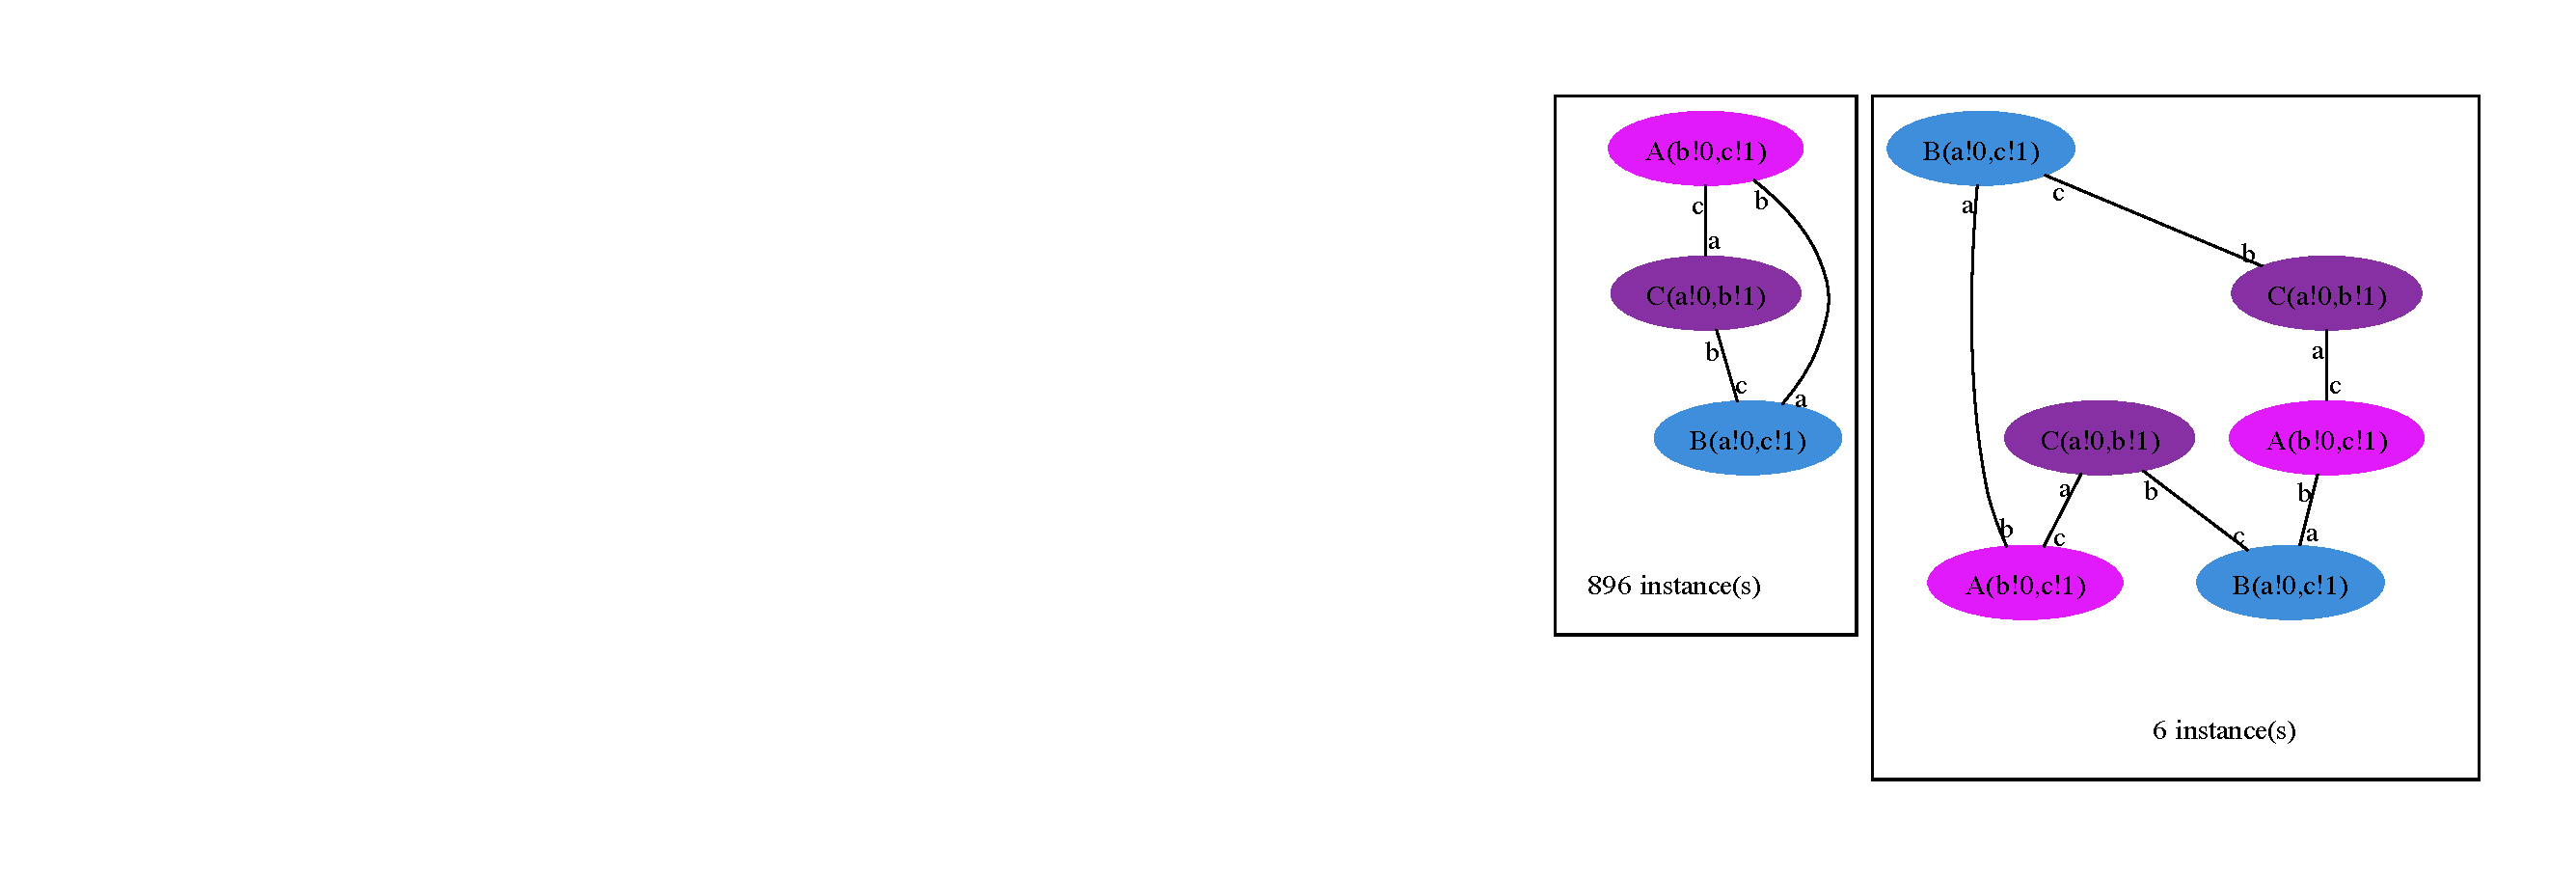
\includegraphics[width=10cm]{img/poly.pdf}
\caption{Final mixture obtained after 10,000 events of simulation of the \ttt{poly.ka} model. The infinite rate for cycle closure allows one to obtain a large number of triangles.}
\label{fig:species}
\end{center}
\end{figure}


\section{Variables}\label{sec:var}

In the KF it is also possible to declare \emph{variables}\index{variable} by a line of the form
\ITE{
\item[] \ttt{\%var: `var\_name'} (\textit{variable\_expression} or \textit{kappa\_expression})
}
where \ttt{var\_name} can be any string and \textit{variable\_expression} is any algebraic expression\index{algebraic expression} on variable names (other than \ttt{var\_name})  using predefined operators summarized in Table~\ref{tab:operators}.

\begin{table}[htbp]
\centering
\begin{tabular}{@{} l|l @{} }
\toprule
Symbol & Interpretation \\
\midrule
\ttt{[E]} & the total number of simulation events\index{event}\\
& since the beginning of the simulation \\
\ttt{[E+]} & the total number of productive events\index{event} \\
\ttt{[E-]} & the total number of null events\index{event}\\
\ttt{[emax]} & the max (productive) event limit as set by the option \ttt{-e}. \\ &Note that if unset \ttt{emax}$=\infty$\\
\ttt{[T]} & the bio-time of the simulation \\
\ttt{[Tsim]} & the cpu-time since the beginning of the simulation \\
\ttt{[tmax]} & the max (bio)-time limit as set by the option \ttt{-t}. \\ &Note that if unset \ttt{tmax}$=\infty$\\

\ttt{`v'} & the value of variable {\ttt `v'} (declared using the \ttt{\%var:} statement) \\
\ttt{[}$f$\texttt{]} & the intuitive mathematical function or constant \\ &associated to $f\in\set{\hbox{\ttt{log,sin,cos,tan,sqrt,pi}}}$ \\
\ttt{[inf]} & symbol for $\infty$ \\
\ttt{[mod]} & the \emph{modulo} operator (infix notation)\\
\ttt{[exp]} & the exponentiation operation $x\mapsto e^x$ \\
\ttt{[int]} & the floor function $x\in\Real\mapsto \lfloor x\rfloor\in\Nat^+$ \\
\ttt{+,-,*,/,\^} & the corresponding mathematical operators (infix notation)\\
\bottomrule
\end{tabular}\caption{Symbol usable in algebraic expressions\index{algebraic expression}.}
\label{tab:operators}
\end{table}
%%
%%
\noi For instance the declarations
\ITE{
\item[] \ttt{\%var: `homodimer' A(x!1),A(x!1)}
\item[] \ttt{\%var: `aa' `homodimer'/2}
}
define 2 variables, the first one tracking the number of embeddings of \ttt{A(x!1),A(x!1)} in the graph over time, while the second divides this value by 2: the number of automorphisms in \ttt{A(x!1),A(x!1)}. The declaration of a variable acts as a binder in the rest of the KF. Hence variables that are used in the expression of another variable must be declared beforehand. 
\vskip 0.25cm
\noi It is also possible to use algebraic expressions\index{algebraic expression} as kinetic rates\index{kinetic rate} as in
\ITE{
\item[] \ttt{\%var: `k\_on' 1.0E-6 \# per molecule per second}
\item[] \ttt{'ab' A(x),A(x) -> A(x!1),A(x!1) @ `k\_on'/2}
}
%%
\KaSim~may output values of variables in the data file\index{data file} (see option \ttt{-p} in Chapter~\ref{chap:cl}) using plot declaration:
\ITE{
\item[] \ttt{\%plot: `var\_name'}
}
One may use the shortcut: 
\ITE{
\item[] \ttt{\%obs: `var\_name' } \textit{variable\_expression}
}
to declare a variable and at the same time require it to be outputted in the data file\index{data file}. 

\section{Initial conditions}\label{sec:init}

The initial mixture\index{mixture} to which rules in the KF will be applied are declared as
\ITE{
\item[] \ttt{\%init: } \textit{mult} \textit{kappa\_expression}
}
%%
where \textit{mult} is either a positive integer or a variable name pointing to a constant expression (ie. not a $\kappa$ expression). This will add to the initial state of the model \textit{mult} copies of the graph described by the kappa expression. Again the DCDW convention\index{don't care don't write} allows us not to write the complete interface of added agents (the remaining sites will be completed according to the agent's signature). For instance:
\ITE{
\item[] \ttt{\%var: 'n' 1000}
\item[] \ttt{\%init: 'n' (A,A(y\int p)) }
}
will add 1000 instances of \ttt{A} in its default state \ttt{A(x,y\int u,z\int 0)} and 1000 instances of \ttt{A} in state \ttt{A(x,y\int p,z\int 0)}.
Note that \ttt{A} is equivalent to writing \ttt{A()}. As any other declaration, \ttt{\%init} can be used multiple times, and agents will add up to the initial state.

\chapter{A simple model}\label{chap:abc}

We describe below the content of a simple Kappa model and give examples of some typical run\footnote{The corresponding kappa file is included in the distribution of \KaSim, in the directory \ttt{models/}}.

\section{ABC.ka}
{\footnotesize\ttt{
\ENU{
\item \tcb{\#\#\#\# Signatures}
\item \%agent: A(x,c) \tcb{\# Declaration of agent A}
\item \%agent: B(x) \tcb{\# Declaration of B}
\item \%agent: C(x1\int u\int p,x2\int u\int p) \tcb{\# Declaration of C with 2 modifiable sites}
\item \tcb{\#\#\#\# Rules}
\item `a.b' A(x),B(x) -> A(x!1),B(x!1) @ `on\_rate' \tcb{\#A binds B} 
\item `a..b' A(x!1),B(x!1) -> A(x),B(x) @ `off\_rate' \tcb{\#AB dissociation} 
\item 'ab.c' A(x!\_,c),C(x1\int u) ->A(x!\_,c!2),C(x1\int u!2)  @ `on\_rate' \tcb{\#AB binds C} 
\item 'mod x1' C(x1\int u!1),A(c!1) ->C(x1\int p),A(c)  @ `mod\_rate' \tcb{\#ABC modifies x1} 
\item 'a.c' A(x,c),C(x1\int p,x2\int u) -> A(x,c!1),C(x1\int p,x2\int u!1) @ `on\_rate' \tcb{\#A binds C on x2}
\item 'mod x2' A(x,c!1),C(x1\int p,x2\int u!1) -> A(x,c),C(x1\int p,x2\int p) @ `mod\_rate' \tcb{\#A modifies x2} 
\item \tcb{\#\#\#\# Variables}
\item \%var: `on\_rate' 1.0E-4 \tcb{\# per molecule per second}
\item \%var: `off\_rate' 0.1 \tcb{\# per second}
\item \%var: `mod\_rate' 1 \tcb{\# per second}
\item \%obs: `AB' A(x!x.B)
\item \%obs: `Cuu' C(x1\int u,x2\int u)
\item \%obs: `Cpu' C(x1\int p,x2\int u)
\item \%obs: `Cpp' C(x1\int p,x2\int p)
\item \tcb{\#\#\#\# Initial conditions}
\item \%init: 1000 A,B
\item \%init: 10000 C
}
}}
%

Line 1-4 of this KF contains signature declarations\index{signature}. Agents of type \ttt{C} have 2 sites \ttt{x1} and \ttt{x2} whose internal state may be \ttt{u}(nphosphorylated) or \ttt{p}(hosphorylated). Recall that the default state of these sites is \ttt{u} (the first one). Line 8, rule \ttt{`ab.c'} binds an \ttt{A} connected to someone on site \ttt{x} (link type \ttt{!\_}) to a \ttt{C}. Note that the only rule that binds an agent to \ttt{x} of \ttt{A} is \ttt{`a.b'} at line 6. Hence the use of \ttt{!\_} is a commodity and the rule could be replaced by 
\ITE{
\item[]\ttt{`alt\_ab.c' A(x!1,c),B(x!1),C(x1\int u) $\rar\dots$}
}
There are two main points to notice about this model: \ttt{A} can modify both sites of \ttt{C} once it is bound to them. However, only an \ttt{A} bound to a \ttt{B} can connect on \ttt{x1} and only a free \ttt{A} can connect on \ttt{x2}. Note also that \ttt{x2} is available for connection only when \ttt{x1} is already modified. 

\section{Some runs}
We try first a coarse simulation of $100,000$ events (10 times the number of agents in the initial system).
\ttt{
\ITE{
\item[\$] KaSim -i ABC.ka -e 100000 -p 1000 -o abc.out
}}
Plotting the content of the \ttt{abc.out} file one notices that nothing of significant interest happen to the observables after 250s. So we can now specify a meaningful time limit by running
\ttt{
\ITE{
\item[\$] KaSim -i ABC.ka -e 100000 -t 250 -p 1000 -o abc.out
}}
which produces the data points whose rendering is given in Fig.~\ref{fig:abc}.
\begin{figure}[htbp]
\begin{center}
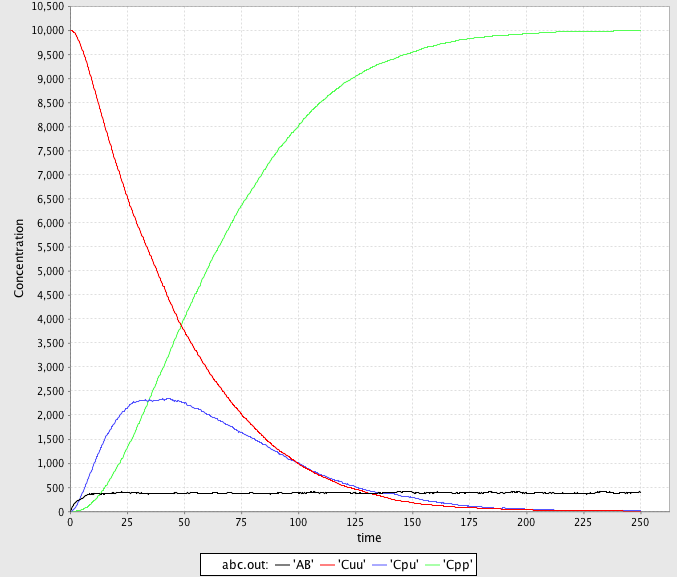
\includegraphics[width=12cm]{img/plot-abc.png}
\caption{Simulation of the ABC model: population of unmodified \ttt{C}s (observable \ttt{Cuu} in red) drops rapidly and is replaced, in a first step by simply modified \ttt{C}s (observable \ttt{Cpu} in blue) which are in turn replaced by doubly modified \ttt{C}s (observable \ttt{Cpp} in red). Note that the population of \ttt{AB} complexes (observable \ttt{AB} in black) stabilizes slightly below 400 individuals after about 20s.}
\label{fig:abc}
\end{center}
\end{figure}
We will use this model as a running example for the next chapter, in order to illustrate various advanced concepts.

\chapter{Advanced concepts}\label{chap:advanced}

\section{Perturbation language}\label{sec:mod}

\subsection{Syntax} 
It is possible to use variables\index{variable} of the model as precondition for triggering a \emph{perturbation}\index{perturbation} of the simulation. For instance one may want to interrupt the simulation whenever a certain amount of observable has been reached, introduce a signal at some time interval etc. To do so, one declares a perturbation with a line:
\ITE{
\item[] \ttt{\%mod:} \textit{boolean\_expression} \ttt{do} \textit{effect} \textit{end\_expression}
}
where \textit{boolean\_expression} and \textit{effect} are defined by the grammar given in Table~\ref{tab:pert}.
%%
\begin{table}[htbp]
  \centering
  \begin{tabular}{@{} lcl @{}}
    \textit{boolean\_expression} &::=& \textit{algebraic\_expression}\index{boolean expression} \tcb{rel} \textit{algebraic\_expression} \\
    && | (\textit{boolean\_expression} \tcb{||} \textit{boolean\_expression}) \\
    && | (\textit{boolean\_expression} \tcb{\&\&} \textit{boolean\_expression}) \\
    && | \tcb{[not]} \textit{boolean\_expression} \\
    && | \tcb{[true]} | \tcb{[false]} \\\\
    \textit{effect} &::=& \tcb{\$ADD} \textit{algebraic\_expression agent\_expression} \\
    && | \tcb{\$DEL} \textit{algebraic\_expression agent\_expression} \\
    && | \tcb{\$SNAPSHOT} | \tcb{\$STOP} \\ && | \tcb{`rule\_name' :=} \textit{algebraic\_expression} \\
    && | \tcb{\$TRACK} \textit{observable} \\\\
    \textit{observable} &::=& \tcb{`rule\_name'} | \tcb{`var\_name'} \\\\
    \textit{end\_expression} &::=& $\varepsilon$ | \tcb{until} \textit{boolean\_expression}
    \end{tabular}
  \caption{Perturbation expressions. The operator \ttt{rel} can be any usual binary relation in $\set{<,=,>}$ and algebraic expressions are built using table~\ref{tab:operators}.}
  \label{tab:pert}
\end{table}
%%
\subsection*{Precondition}
Basically, the \textit{precondition}\index{precondition} determines when the perturbation will be triggered, for instance a user writes
\ITE{
\item[] \ttt{\%mod: ([T]>10) \&\& (`v1'/`v2') > 1 do $\dots$}
}
to indicate she wishes to trigger a perturbation whenever the simulation time has passed 10 time units and the ratio of variables \ttt{v1} over \ttt{v2} is above 1. Note that the perturbations are by default "one shot" interventions in the simulation. Once the precondition is satisfied, the perturbation is applied and discarded, unless a persistent perturbation is used using the \ttt{until} keyword (see below). 

\subsection*{Effect}

The \textit{effect} of a perturbation can be divided in two kinds: the perturbations that modify the mixture, and those that simply give modelers an additional insight of what is going on in the simulation.

In the first kind one may add (\ttt{\$ADD} instruction), delete (\ttt{\$DEL} instruction) agents from the mixture or modify the kinetic rate\index{kinetic rate} of a particular rule. In the second category one may record the current state of the mixture (\ttt{\$SNAPSHOT} instruction), interrupt the simulation in order to save the current state (\ttt{\$STOP} instruction) or decide to trigger some causality analysis on some particular observable of interest (\ttt{\$TRACK} instruction)\index{causality analysis}.

\subsection*{Persistent perturbation}
The \textit{end\_expression} serves to specify whether the perturbation should be applied only once ("one shot" perturbation) or at every future events until a condition is reached (persistent perturbation). For instance:
\ttt{\ITE{
\item[] \%mod: ([T] [mod] 100)=0 do \$DEL  [inf] C until [T]>1000
}}
will delete every \ttt{C} from the mixture every 100 t.u until the simulation clock has passed 1000 t.u. If no \ttt{until} keyword is positioned, the perturbation will be discarded after its first application.


\subsection{Modifying the mixture during a simulation}

Continuing with the ABC model, the perturbation effect: 
\ttt{\ITE{
\item[] \$ADD $n$ C(x1\int p)
}}
will add $n\geq 0$ instances of \ttt{C} with \ttt{x1} already in state \ttt{p} (and the rest of its interface in the default state as specified line 4 of ABC.ka). Also the perturbation effect:
\ttt{\ITE{
\item[] \$DEL  [inf] B(x!\_)
}}
will remove \emph{all} \ttt{B}s connected to someone from the mixture. Now, the effect:
\ttt{\ITE{
\item[] `rule\_name' :=  [inf]
}}
will set the kinetic rate of a declared rule named \ttt{`rule\_name'} to $\infty$.

\subsection*{Example}
There are various ways one can use perturbations to study more deeply a given kappa model. A basic illustration is the use of a simple perturbation to let a system equilibrate before starting a real simulation. For instance, as can be seen from the curve given in Fig.~\ref{fig:abc}, the number of AB complexes is arbitrarily set to 0 in the initial state (all \ttt{A}s are disconnected from \ttt{B}s in the initial mixture). In order to avoid this, one can modify the kappa file the following way: we set the initial concentration of \ttt{C} to 0 by deleting line 22. Now we introduce \ttt{C}s after 25 t.u by perturbation:
\ttt{\ITE{
\item[] \%mod:  [T]>25 do \$ADD 10000 C 
}}
The modified kappa file is available in the source repository, in the \ttt{model/} directory (file \ttt{abc-pert.ka}). 
Running again a simulation (a bit longer) by entering in the command line:
\ttt{
\ITE{
\item[\$] KaSim -i ABC-pert.ka -e 100000 -t 300 -o abc2.out
}}
one obtains the curve given in Fig.~\ref{fig:abc2}
\begin{figure}[htbp]
\begin{center}
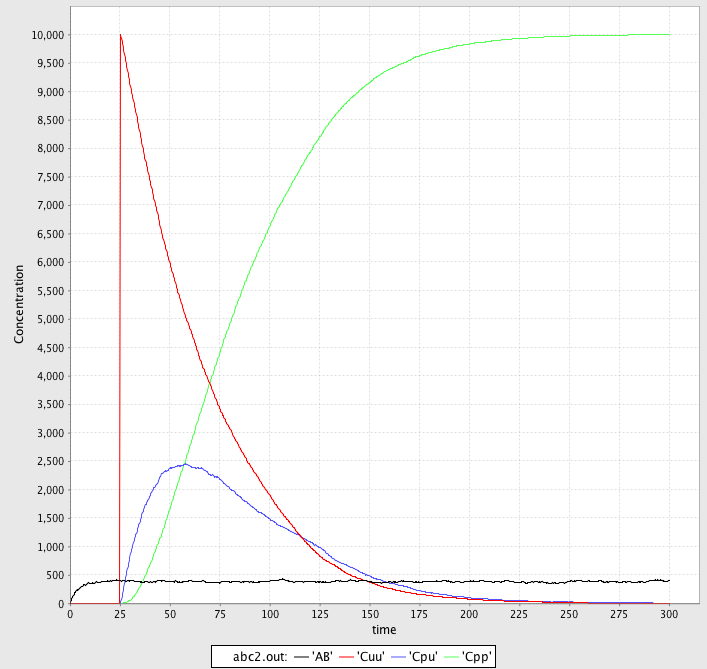
\includegraphics[width=10cm]{img/plot-abc2.png}
\caption{Simulation of the ABC model with a perturbation: for t<25s, only \ttt{`a.b'} and \ttt{`a..b'} rules may apply. This enables the concentration of \ttt{`AB'} complexes to go to steady state, before introducing fresh \ttt{C}s at t=25s.}
\label{fig:abc2}
\end{center}
\end{figure}

\subsection{Snapshots}

In the previous example, we let the system evolve for some time without its main reactant \ttt{C} in order to let other reactants go to a less arbitrary initial state. One may object that this way of proceeding is CPU-time consuming if one has to do this at each simulation. An alternative is to use the \ttt{\$SNAPSHOT} primitive that allows a user to export a snapshot of the mixture at a given time point as a new (piece of) kappa file.
For instance, the declaration:
\ttt{\ITE{
\item[] \%mod:  [E-]/[E]>0.9 do \$SNAPSHOT \textquotedbl prefix\textquotedbl
}}

will ask \KaSim~to export the mixture the first time the ration of null events over productive ones will reach 0.9. The exported file will be named \ttt{prefix\_$n$.ka} where $n$ is the event number at which the snapshot was taken. Note that one may omit to define a prefix and simply type:
\ttt{\ITE{
\item[] \%mod:  [E-]/[E]>0.9 do \$SNAPSHOT
}}
in which case the default prefix \ttt{snap} will be used for naming snapshots.

Note that if the name already exists a counter will be appended at the end of the file to prevent overwriting.
Note that snapshots can be performed multiple times, for instance every 1000 events, using the declaration:
\ttt{\ITE{
\item[] \%mod:  ([E+] [mod] 1000)=0 do \$SNAPSHOT \textquotedbl abc\textquotedbl~until [false] 
}}
which results in \KaSim~producing a snapshot every 1000 (productive) events until the simulation ends. The perturbation \ttt{\$STOP "final\_state"} will terminate the simulation whenever its precondition is satisfied and produce a snapshot of the last mixture. Note that instead of producing kappa files, one may use snapshot perturbations to produce an image of the mixture in the dot format using the parameter \ttt{"dotSnapshots"} (see Section~\ref{sec:param}).

\subsection{Causality analysis}\index{causality analysis}
Causality analysis are always triggered by a perturbation of the form:
\ITE{
\item[] \ttt{\%mod:}  \textit{start\_condition} \ttt{do \$TRACK }\textit{observable} \ttt{until} \textit{end\_condition} 
}
where \textit{start\_condition} and \textit{end\_condition} specify respectively when causality analysis should start and finish (remember that in the absence of \ttt{until} construct, causality analysis will only be performed during one computation event!). The \emph{observable} is either a rule's name \ttt{'r'} or a variable name \ttt{'v'} pointing to a kappa expression. For instance, in the ABC model, the declaration:
\ttt{\ITE{
\item[] \%mod:  [E=0] do \$TRACK 'Cpp' until [false] 
}}
is asking~\KaSim~to track the appearance of the observable \ttt{'Cpp'} since the beginning of the simulation, and display the causal explanation of every new occurrence of \ttt{'Cpp'}, until the end of the simulation. The explanation, that we call \emph{causal flow}\index{causal flow}, is a set of rule application ordered by causality and displayed as a graph using dot format. In this graph, an edge \ttt{r}$\longrightarrow$ \ttt{r'} between two rule applications $\ttt{r}$ and $\ttt{r'}$ indicates that the first rule application has used, in the simulation, some sites that were modified by the application of the former. We show Fig.~\ref{fig:cflow} an example of such causal flow.

\begin{figure}[htbp]
\begin{center}
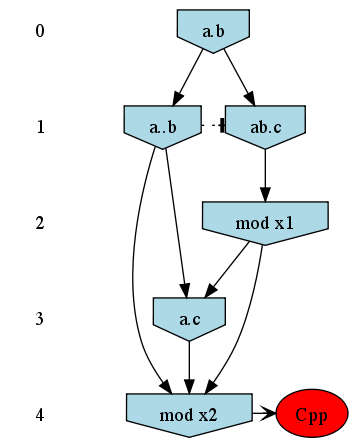
\includegraphics[width=5cm]{img/cflow.png}
\caption{Causal flow for the observable \ttt{'Cpp'} of the ABC model. Plain arrows represent causal dependency, dotted arrows show asymmetric conflict between rule occurrences. Here the \ttt{'ab.c'} rule has to occur before the \ttt{'a.b'} rule. Red observable indicate that the last rule allowed one to observe a new instance of \ttt{'Cpp'}.}
\label{fig:cflow}
\end{center}
\end{figure}

Note that causal flow can show or hide more causal dependencies using various compression techniques that can be enabled as a simulation parameter (see Section~\ref{sec:param}). 

\section{Link type}

In standard kappa, in order to require a site to be bound for an interaction to occur, one may use the \emph{semi-link}\index{semi-link} construct \ttt{!\_} which does not specify who the partner of the bond is. For instance in the variable:
\ttt{\ITE{
\item[] \%var: 'ab' A(x!\_),B(y!\_)
}}
will count the number of \ttt{A}s and \ttt{B}s connected to someone, including the limit case \ttt{A(x!1),B(y!1)}. It is sometimes convenient to specify the \emph{type}\index{link type} of the semi-link, in order to restrict the choice of the binding partner. For instance the variable:
\ttt{\ITE{
\item[] \%var: 'ab' A(x!y.B),B(y!x.A)
}}
will count the number of \ttt{A}s whose site \ttt{x} is connected to a site \ttt{y} of \ttt{B}, plus the number of \ttt{B}s whose site \ttt{y} is connected to a site \ttt{x} of \ttt{A}. Note that this still includes the case \ttt{A(x!1),B(y!1)}.

\section{Implicit signature}
\KaSim~permits users in a hurry to avoid writing agent signatures explicitly using the option \ttt{-\,-implicit-signature} of the command line. The signature is then deduced using information gathered in the KF. Note that it is not recommended to use the DCDW convention for introduced agents in conjunction with the \ttt{-\,-implicit-signature} option unless the default state of all sites is mentioned in the \ttt{\%init} declarations or in the rules that create agents. 

\section{Influence map}
The influence map of a model is an object that may help modelers checking the consistency of the rule set they use. It is generated by the command:
\ttt{\ITE{
\item [] KaSim -i abc.ka -im map.dot -e 0
}}
\noi This will generate the so called \emph{influence map}\index{influence map} of the \ttt{abc.ka} file (the option \ttt{-e 0} specifies that no simulation should be run).
The influence map is statically computed and does not depend on kinetic rates nor initial conditions. It describes how rules \emph{with no side effect}\index{side effect} may potentially influence each other during a simulation. \KaSim~will produce a dot format file containing the influence relation over all rules and observables of the model. The produced graph visualized using a circular rendering\footnote{One may use for instance the \ttt{circo} program that is part of the \textit{graphviz} suite.} is given in Figure~\ref{fig:abc-im}. Observables are represented as circular nodes\footnote{Observable can be viewed as identity rules for computing influence.} and rules as rectangular nodes. Edges are decorated with the list of embeddings (separated by a semi-colon) allowing rules's right hand sides to be mapped to left hand sides. Note that the influence map will not display relations between rules that are induced by side effects (see Section~\ref{sec:side-effect}).

\begin{figure}[htbp] %  figure placement: here, top, bottom, or page
   \centering
   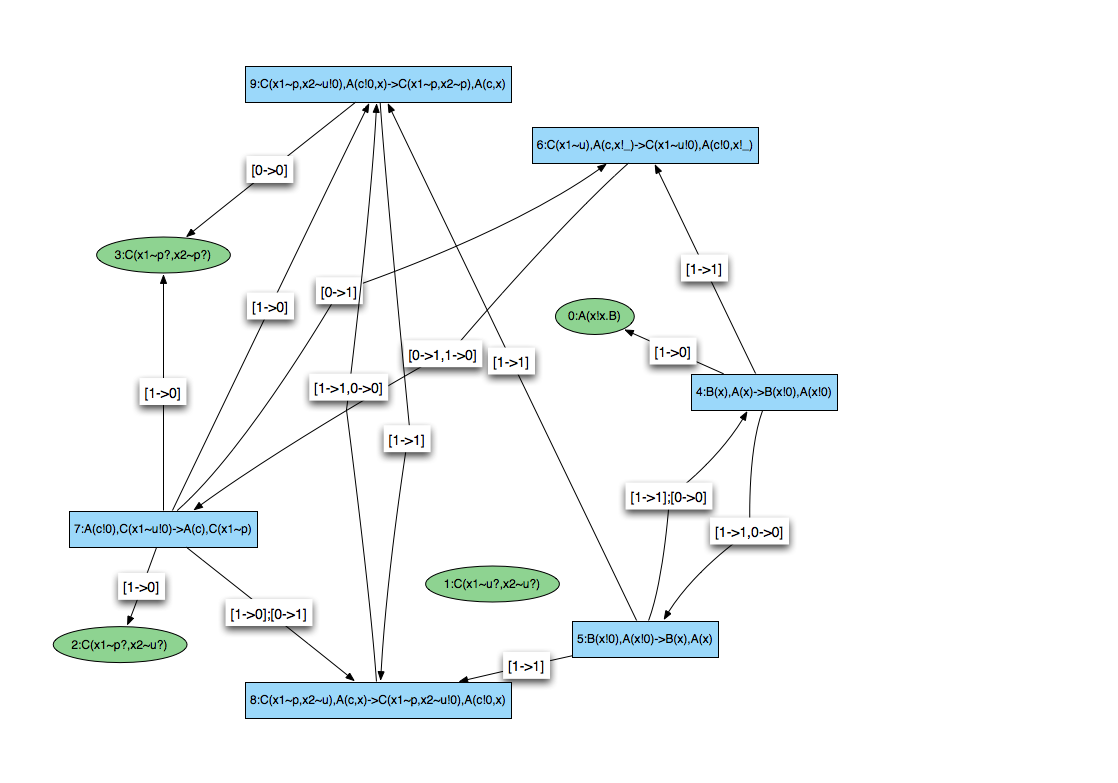
\includegraphics[width=19cm]{img/abc-im.png} 
   \caption{The influence map of the \ttt{abc.ka} model defined in Chapter~\ref{chap:abc}. Note that observable \ttt{C(x1\int u?,x2\int u?)} is not activated by any other rule. This implies that its number of occurrences does not change during a simulation. Edge labels denote embeddings with the convention that $[i\rar j]$ denotes the embedding of agent number $i$ of the origin's rhs, into agent $j$ of the target's lhs.}
   \label{fig:abc-im}
\end{figure}

More formally, consider the rules $r:L\rar R$ and $s:L'\rar R'$. One wishes to know whether it is possible that the application of rule $r$ over a graph $G$ creates a new instance of rule $s$. To do so, \KaSim~will try to generate a $\ka$-term $T$ containing a match for $R$ and $L'$ that overlap on some sites that are modified by $r$ (see Figure~\ref{fig:im} for illustration).

\begin{figure}[htbp] %  figure placement: here, top, bottom, or page
   \centering
   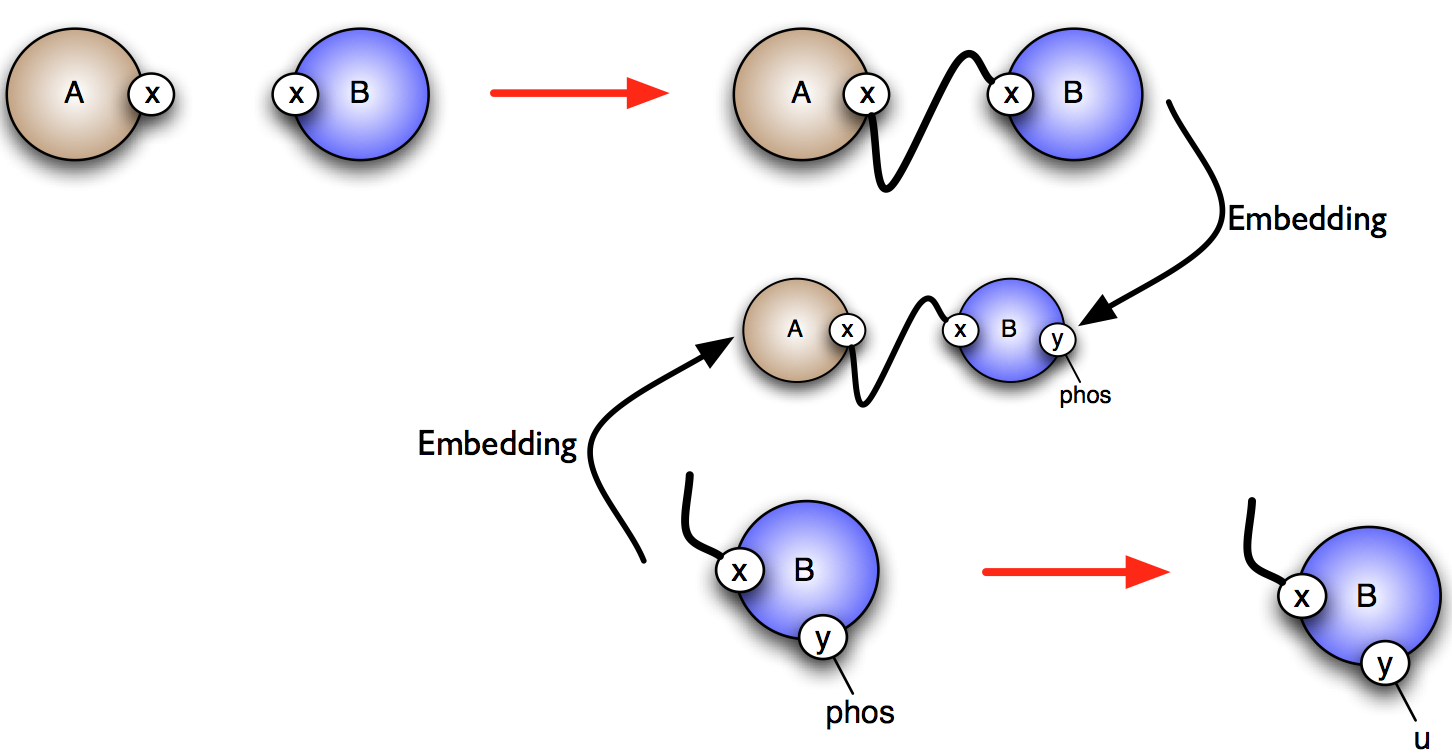
\includegraphics[width=10cm]{img/im.png} 
   \caption{Computation of the influence of the top rule on the rule below: the right hand side of the first rules embeds in a common term with the left hand side of the second rule. It results that the first rule has a positive influence on the second.}
   \label{fig:im}
\end{figure}

\section{Flux map}
The \emph{flux map} is a powerful observation that tracks on the fly the influence rule applications have on each other. Contrary to the influence map, it is dynamically generated and tracks effective impacts (positive or negative) a every rule application. The flux map is obtained by the command:
\ttt{\ITE{
\item [] KaSim -i abc.ka -im map.dot -t $n$
}}
The resulting \emph{flux map} is a graph where a positive edge between rules $r$ and $s$ (in green) indicates an overall positive contribution of $r$ over $s$. Said otherwise, the sum of $r$ applications increased the activity\index{activity} of $s$. Conversely, a negative edge (in red) will indicate that $r$ had an overall negative impact on the activity\index{activity} of $s$. Note that visualization software permitting the importance of the flux between two rules can be observed by looking at the label on the edges that indicate the overall activity transfer (positive or negative) between the rules. An example of flux map is given in Fig.~\ref{fig:flux}. Note that flux may vary during time, therefore the time or event limit of the simulation is of importance and will likely change the aspect of the produced map.

\begin{figure}[htbp] %  figure placement: here, top, bottom, or page
   \centering
   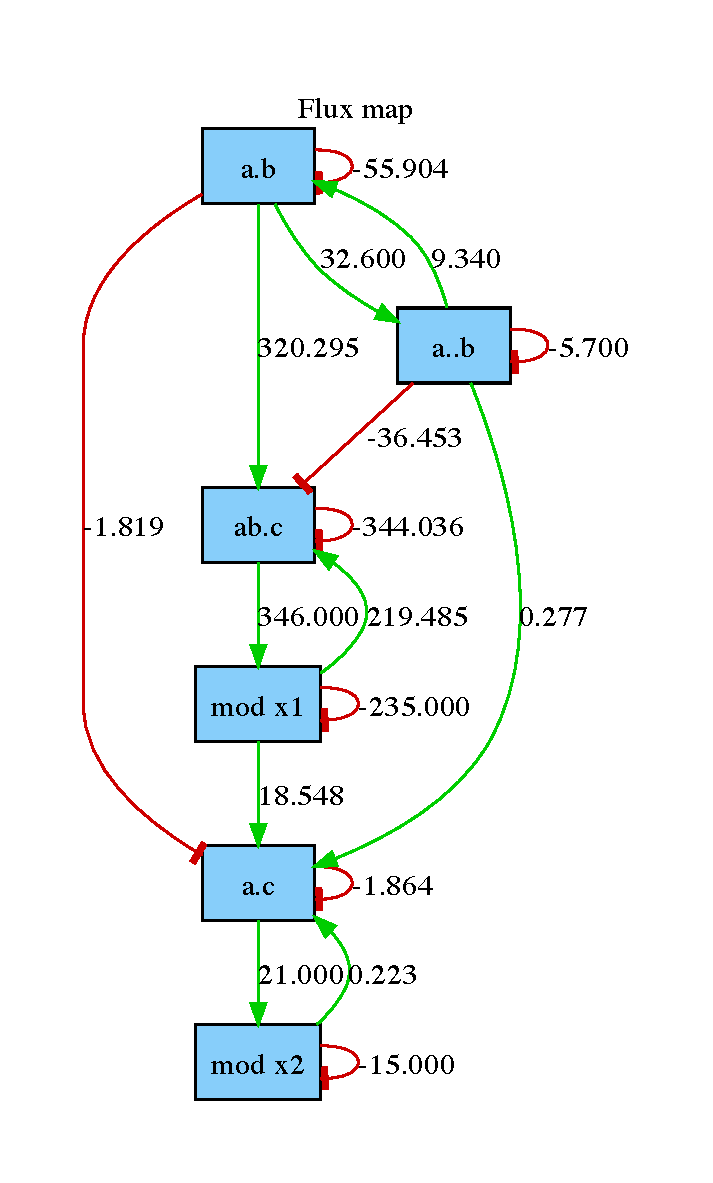
\includegraphics[width=7cm]{img/flux.pdf} 
   \caption{Flux map of the \ttt{abc.ka} model, taken from t=0 to t=20 time units. The \ttt{A} releasing rules \ttt{a..b} and \ttt{mod x2} are contributing very little to the activity of \ttt{a.c} which is a sign of an excess of free \ttt{A}s in the system at this time interval.}
   \label{fig:flux}
\end{figure}

\section{Simulation packages}

The simulation algorithm that is implemented in \KaSim~requires an initialization phase whose complexity is proportional to $R*G$ where $R$ is the cardinal of the rule set and $G$ the size of the initial mixture\index{mixture}. Thus for large systems, initialization may take a while. Whenever a user wishes to run several simulations of the \emph{same} kappa model, it is possible to skip this initialization phase by creating a \emph{simulation package}\index{simulation package}. For instance:
\ttt{\ITE{
\item [] KaSim -i abc.ka -t $n$ -make-sim abc.kasim
}}
will generate a standard simulation of the \ttt{abc.ka} model, but in addition, will create the simulation package \ttt{abc.kasim} (.kasim extension is not mandatory). This package is a binary file, \ie not human readable, that can be used as input of a new simulation using the command:
\ttt{\ITE{
\item [] KaSim -load-sim abc.kasim -t $k$ 
}}
Note that this simulation is now run for $k$ time units instead of $n$. Importantly, simulation packages can only be given as input to the \emph{same} \KaSim~that produced it. As a consequence, recompiling the code, or obtaining different binaries, will cause the simulation package to become useless.

\section{Simulation parameters configuration}\label{sec:param}
In the KF (usually in a dedicated file) one may use expressions of the form:
\[
\hbox{\ttt{\%set: "}\textit{parameter\_name}\ttt{" "}\textit{parameter\_value}\ttt{"}}
\]
where tunable parameters are described table~\ref{tab:parameters}.
%%
\begin{table}[ht]
\begin{tabular}{l|l|lll}
parameter & possible values & description \\
\hline &\\
\textit{Causality analysis}&\\
\ttt{"compressionMode"} & \ttt{"none", "strong", "weak"} & \small type of compression \\
\ttt{"cflowFileName"} & \ttt{"cflow.dot"} or any string & \small file name for causal flows\\ & \\
\textit{Pretty printing}&\\
\ttt{"plotSepChar"} & \ttt{" "} or any character & \small separation character for plots\\
\ttt{"dotSnapshots"} & \ttt{"false", "true"} & \small generate dot snapshots\\
\ttt{"colorDot"} &  \ttt{"false", "true"} & \small use colors in dot format files\\
\ttt{"progressBarSymbol"} & \ttt{"\#"} or any character & \small symbol for the progress bar\\
\ttt{"progressBarSize"} & \ttt{"60"} or any integer & \small length of the progress bar\\ &&\\
\textit{Simulation options} &\\
\ttt{"dumpIfDeadlocked"} & \ttt{"false","true} & \small Snapshot when simulation \\&&\small is stalled\\
\ttt{"maxConsecutiveClash"} & \ttt{"2"} or any integer & \small number of consecutive clashes \\ && \small before giving up \\ && \small square approximation\\

\end{tabular}\caption{User defined parameters. Default values are given first in the possible values column.}\label{tab:parameters}
\end{table}
%%

\bibliographystyle{plain}
\bibliography{fmb} 

\printindex

\end{document}  
